\section{Accessibilità}
	\subsection{Schema colori}
	Si è utilizzato il programma \emph{Colour Contrast Analyser} per testare le combinazioni di colore sfondo e primo piano, allo scopo di determinare se sono in grado di fornire un buon livello di visibilità e se la leggibilità del testo su una pagina Web e la leggibilità di una rappresentazione del testo basata su immagini è possibile da tutti.\\
	Inoltre per la scelta dei colori ci si è basati anche su come viene visualizzato il sito da persone con determinati disturbi visivi grazie al sito \url{http://www.color-blindness.com/coblis-color-blindness-simulator/}.\\
	Vengono riportate alcune simulazioni dell'home page per la protanopia, deuteranopia e tritanopia.\\
	
	\centerline{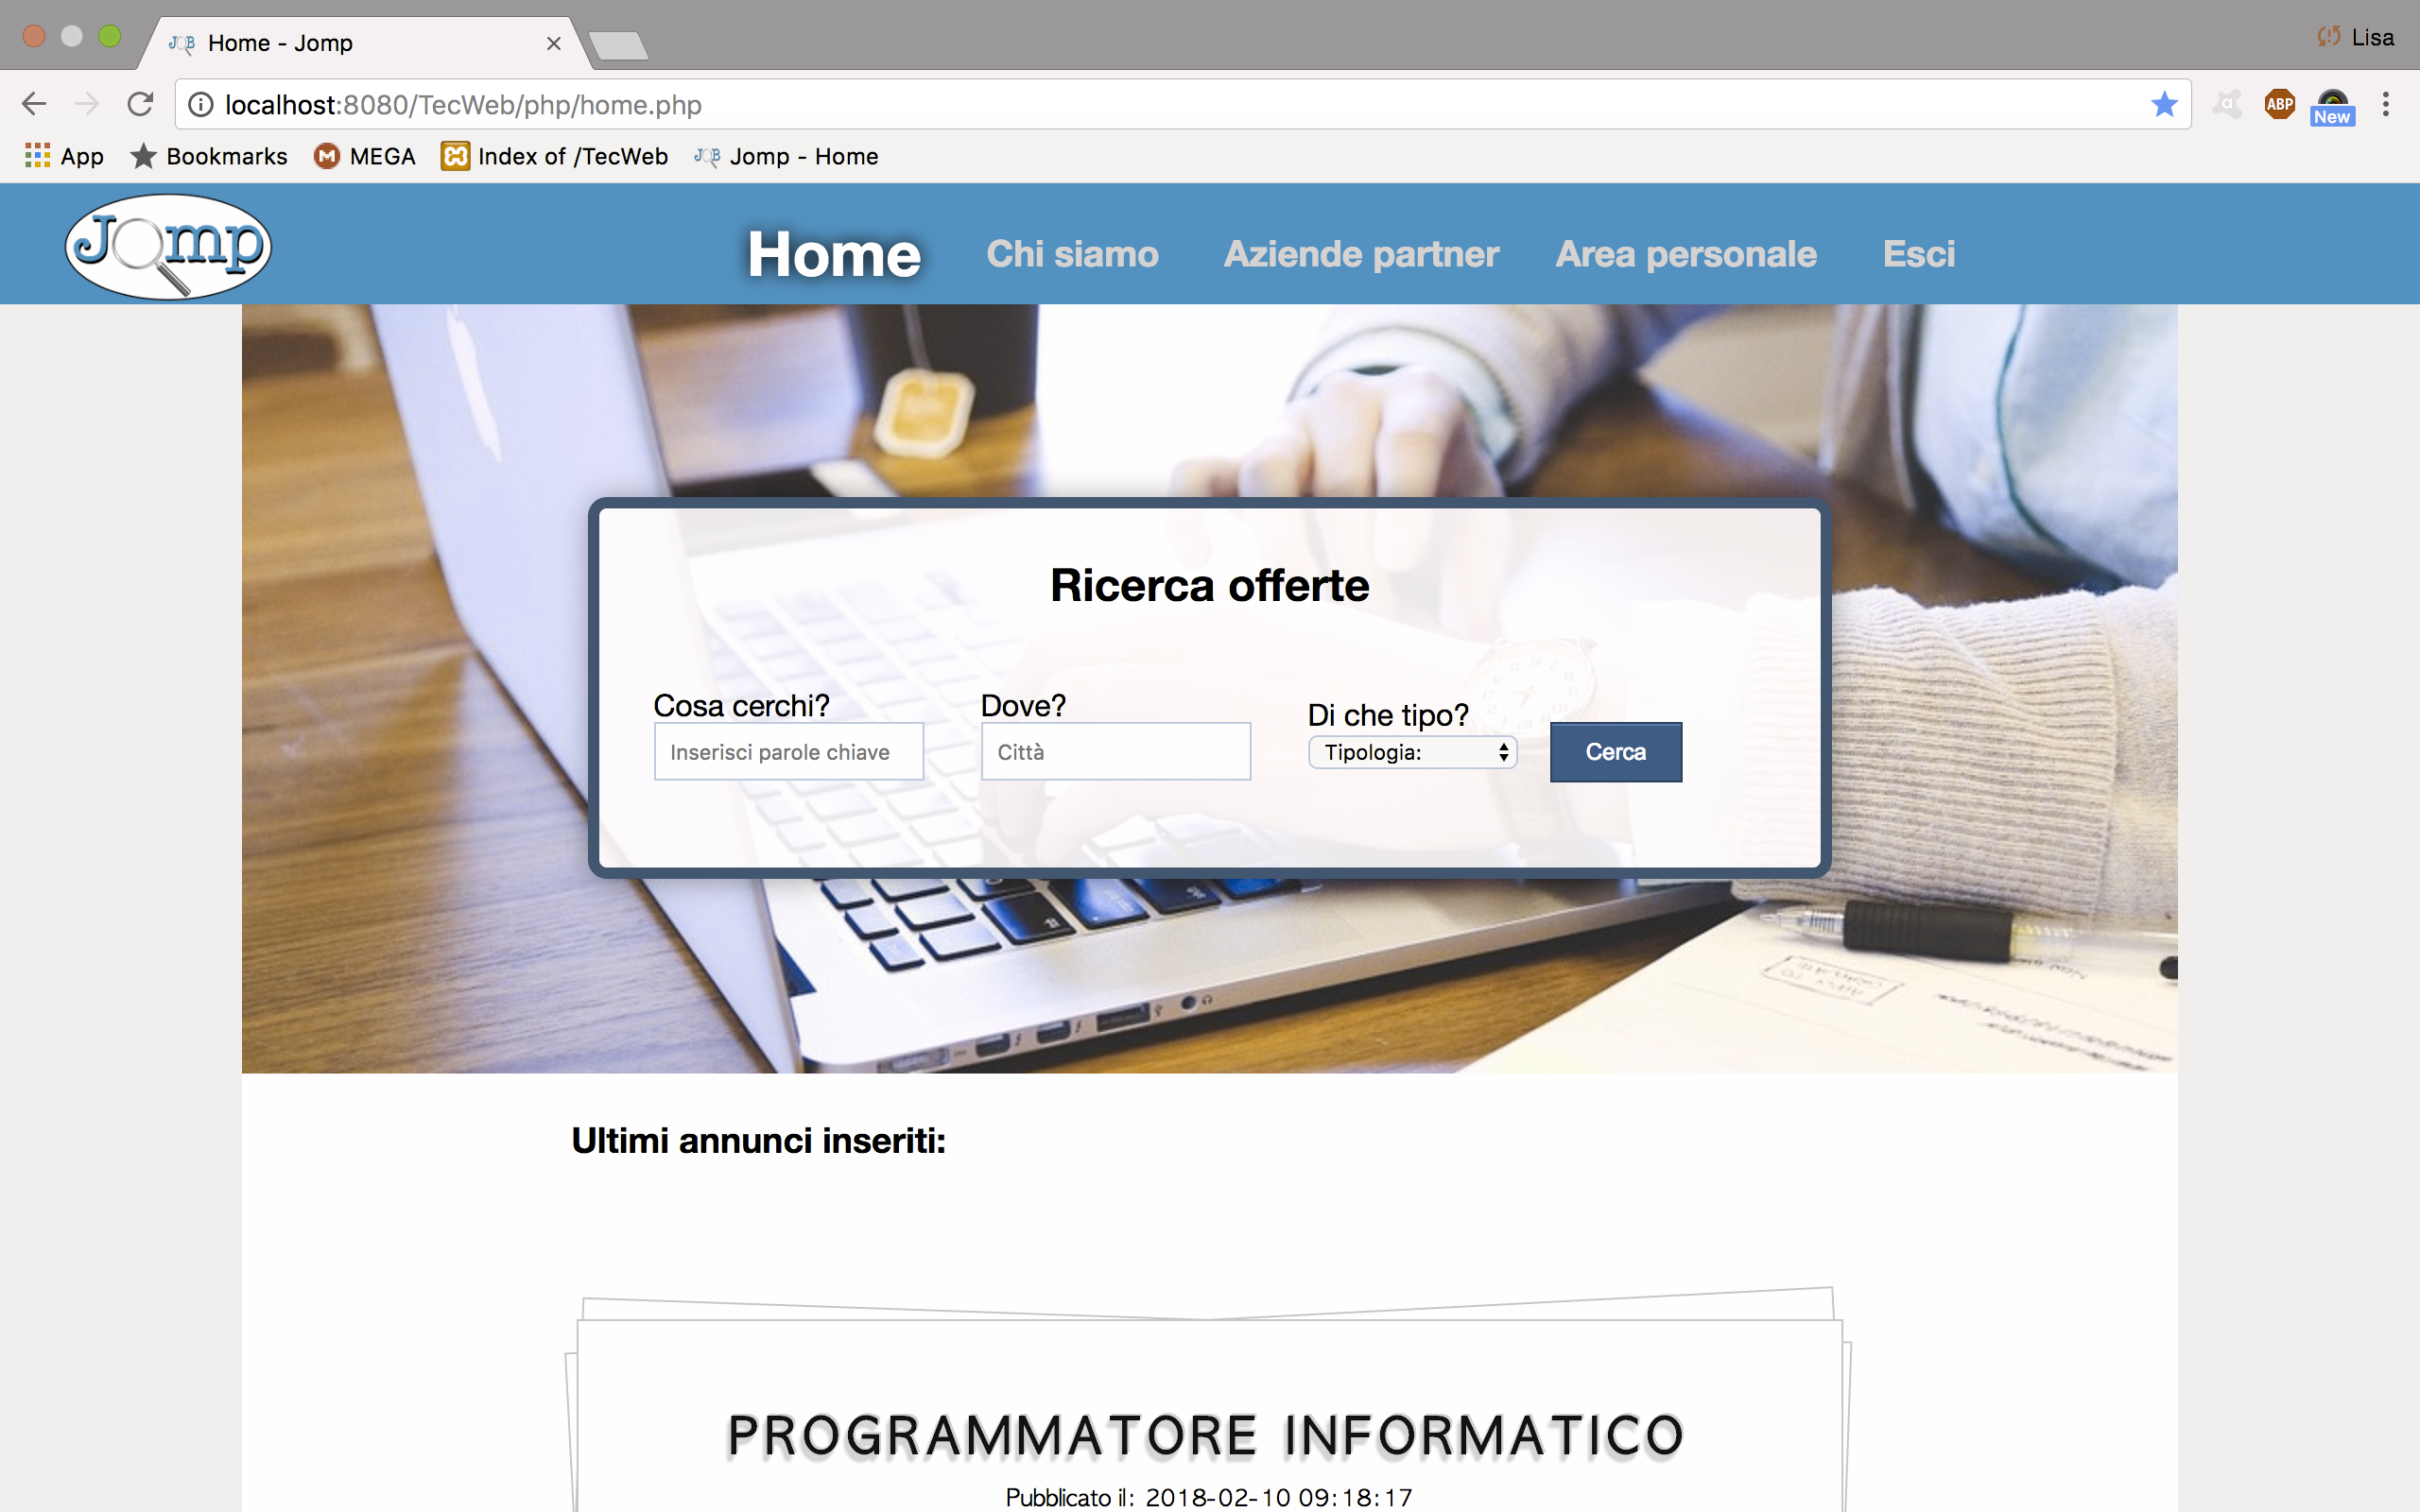
\includegraphics[scale=0.12]{Images/protanopia.jpg}} 
	\vspace{15pt}
	\centerline{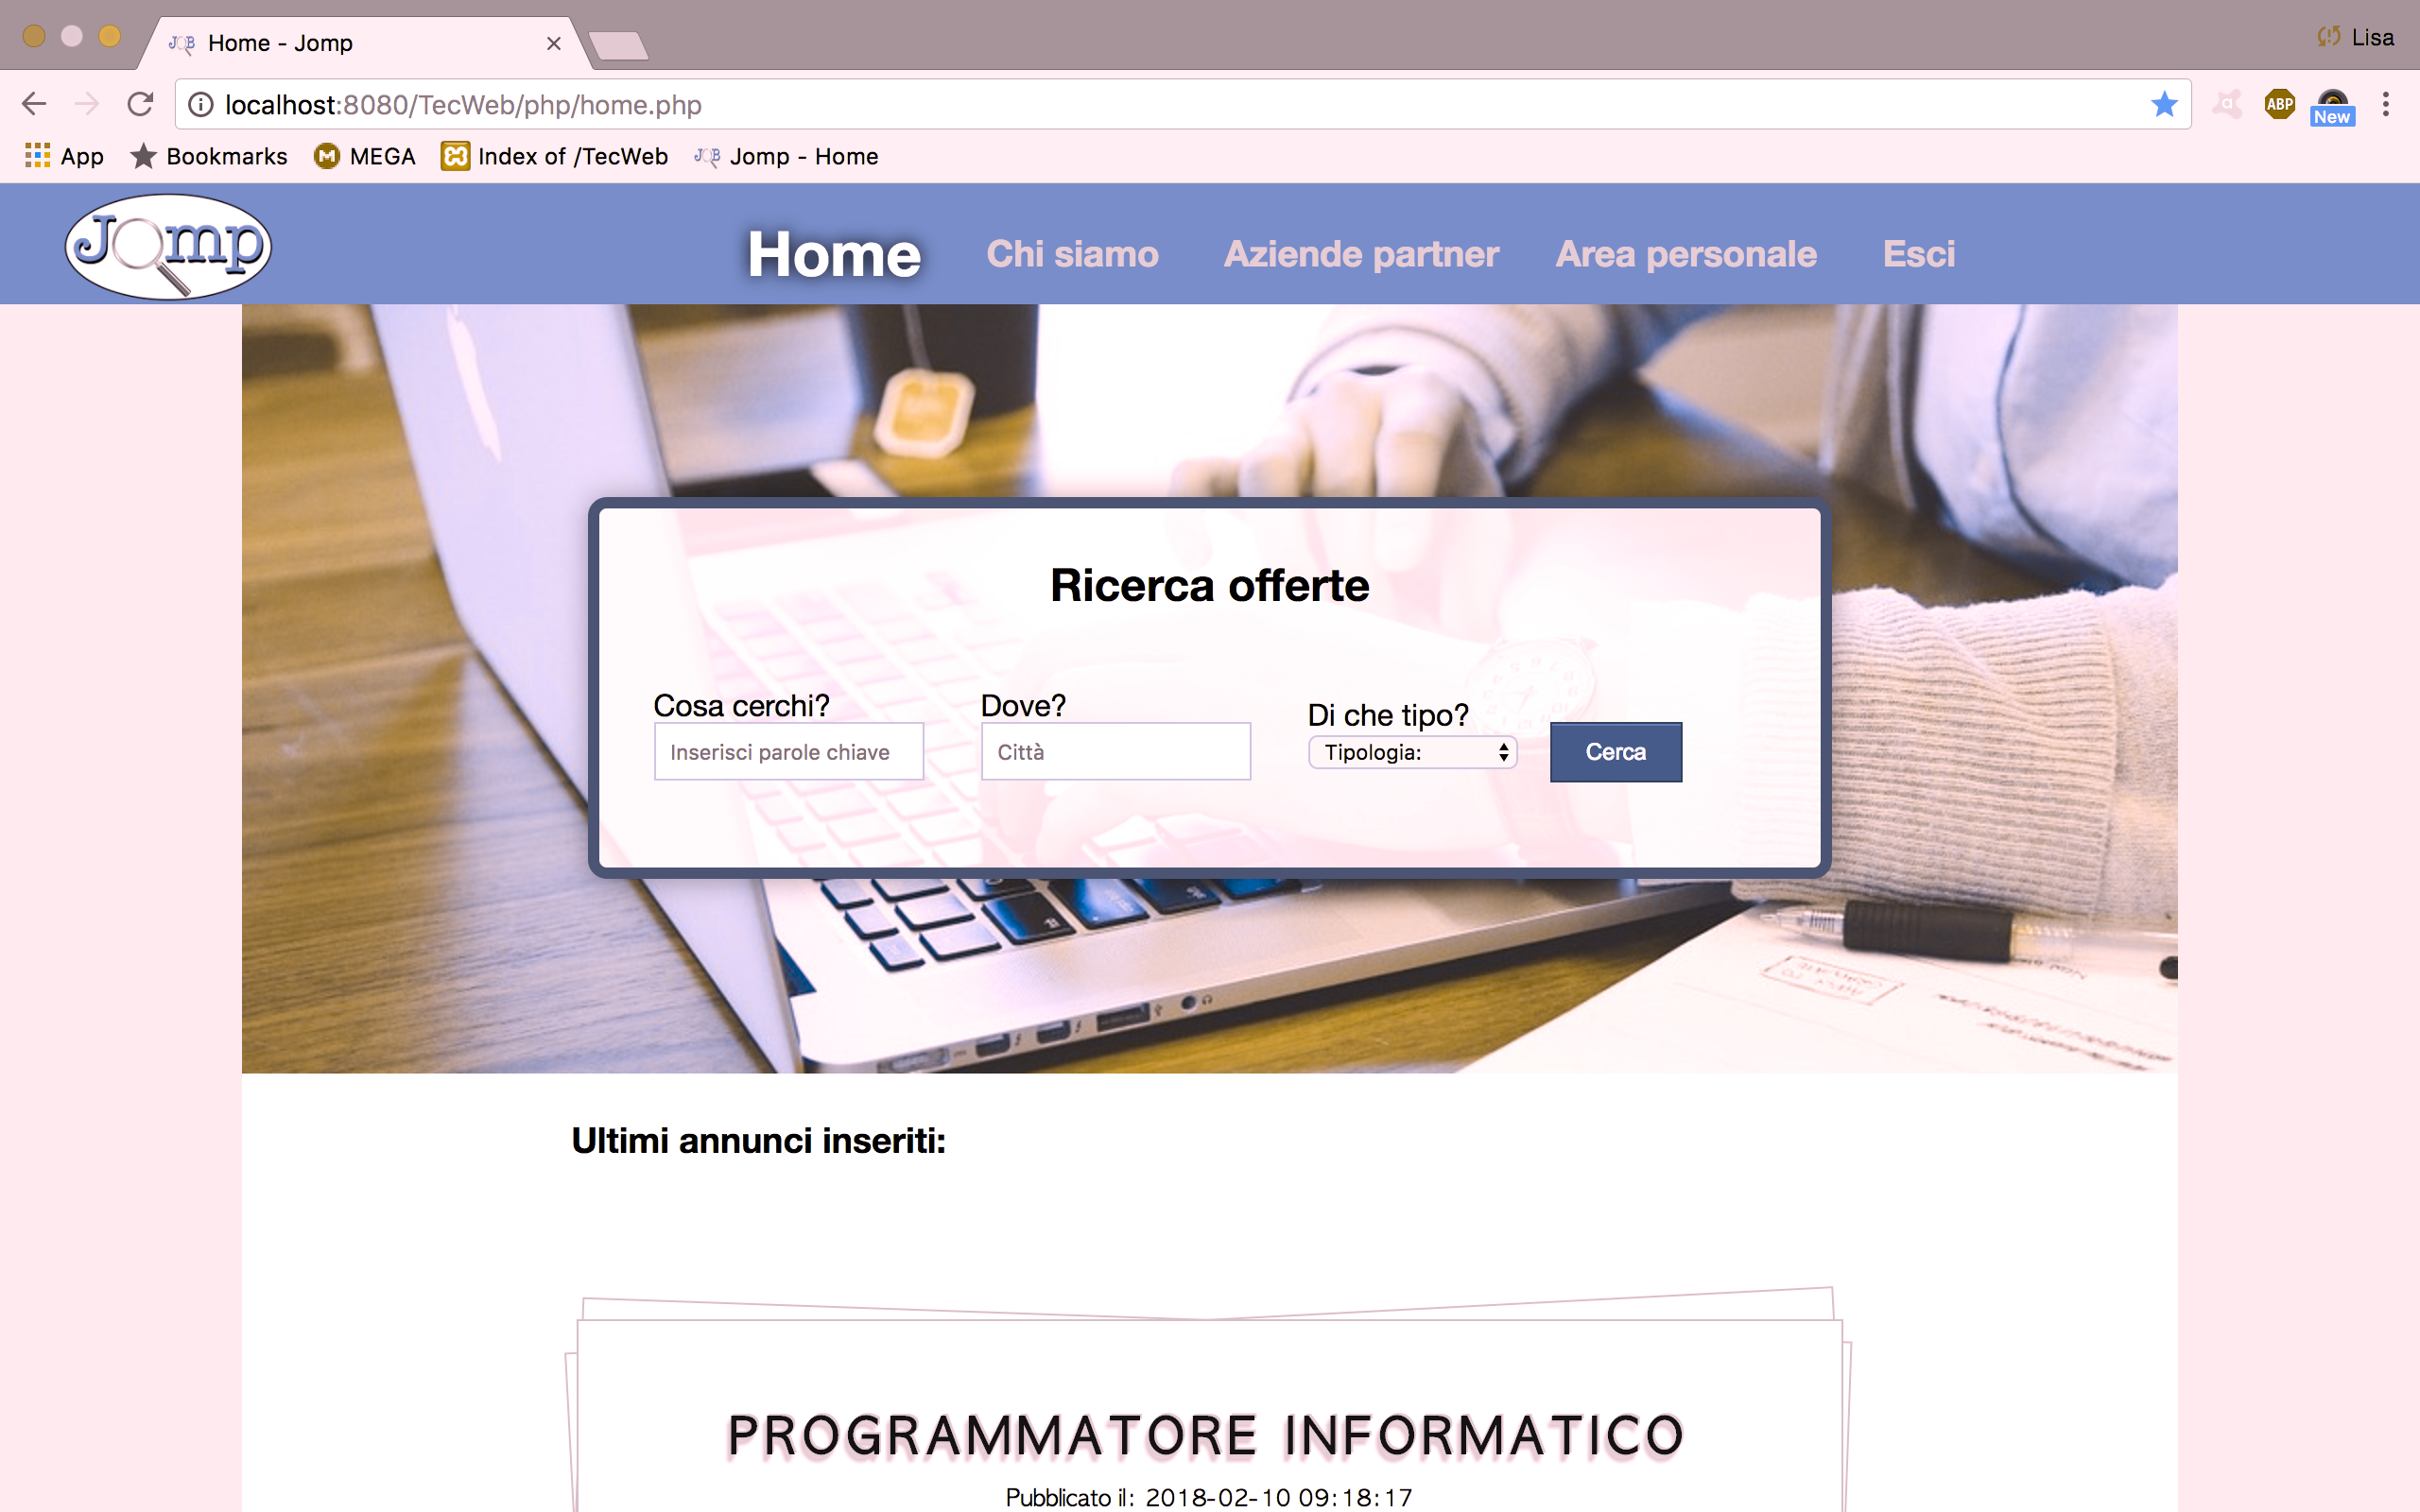
\includegraphics[scale=0.12]{Images/deuteranopia.jpg}}
	\vspace{15pt}
	\centerline{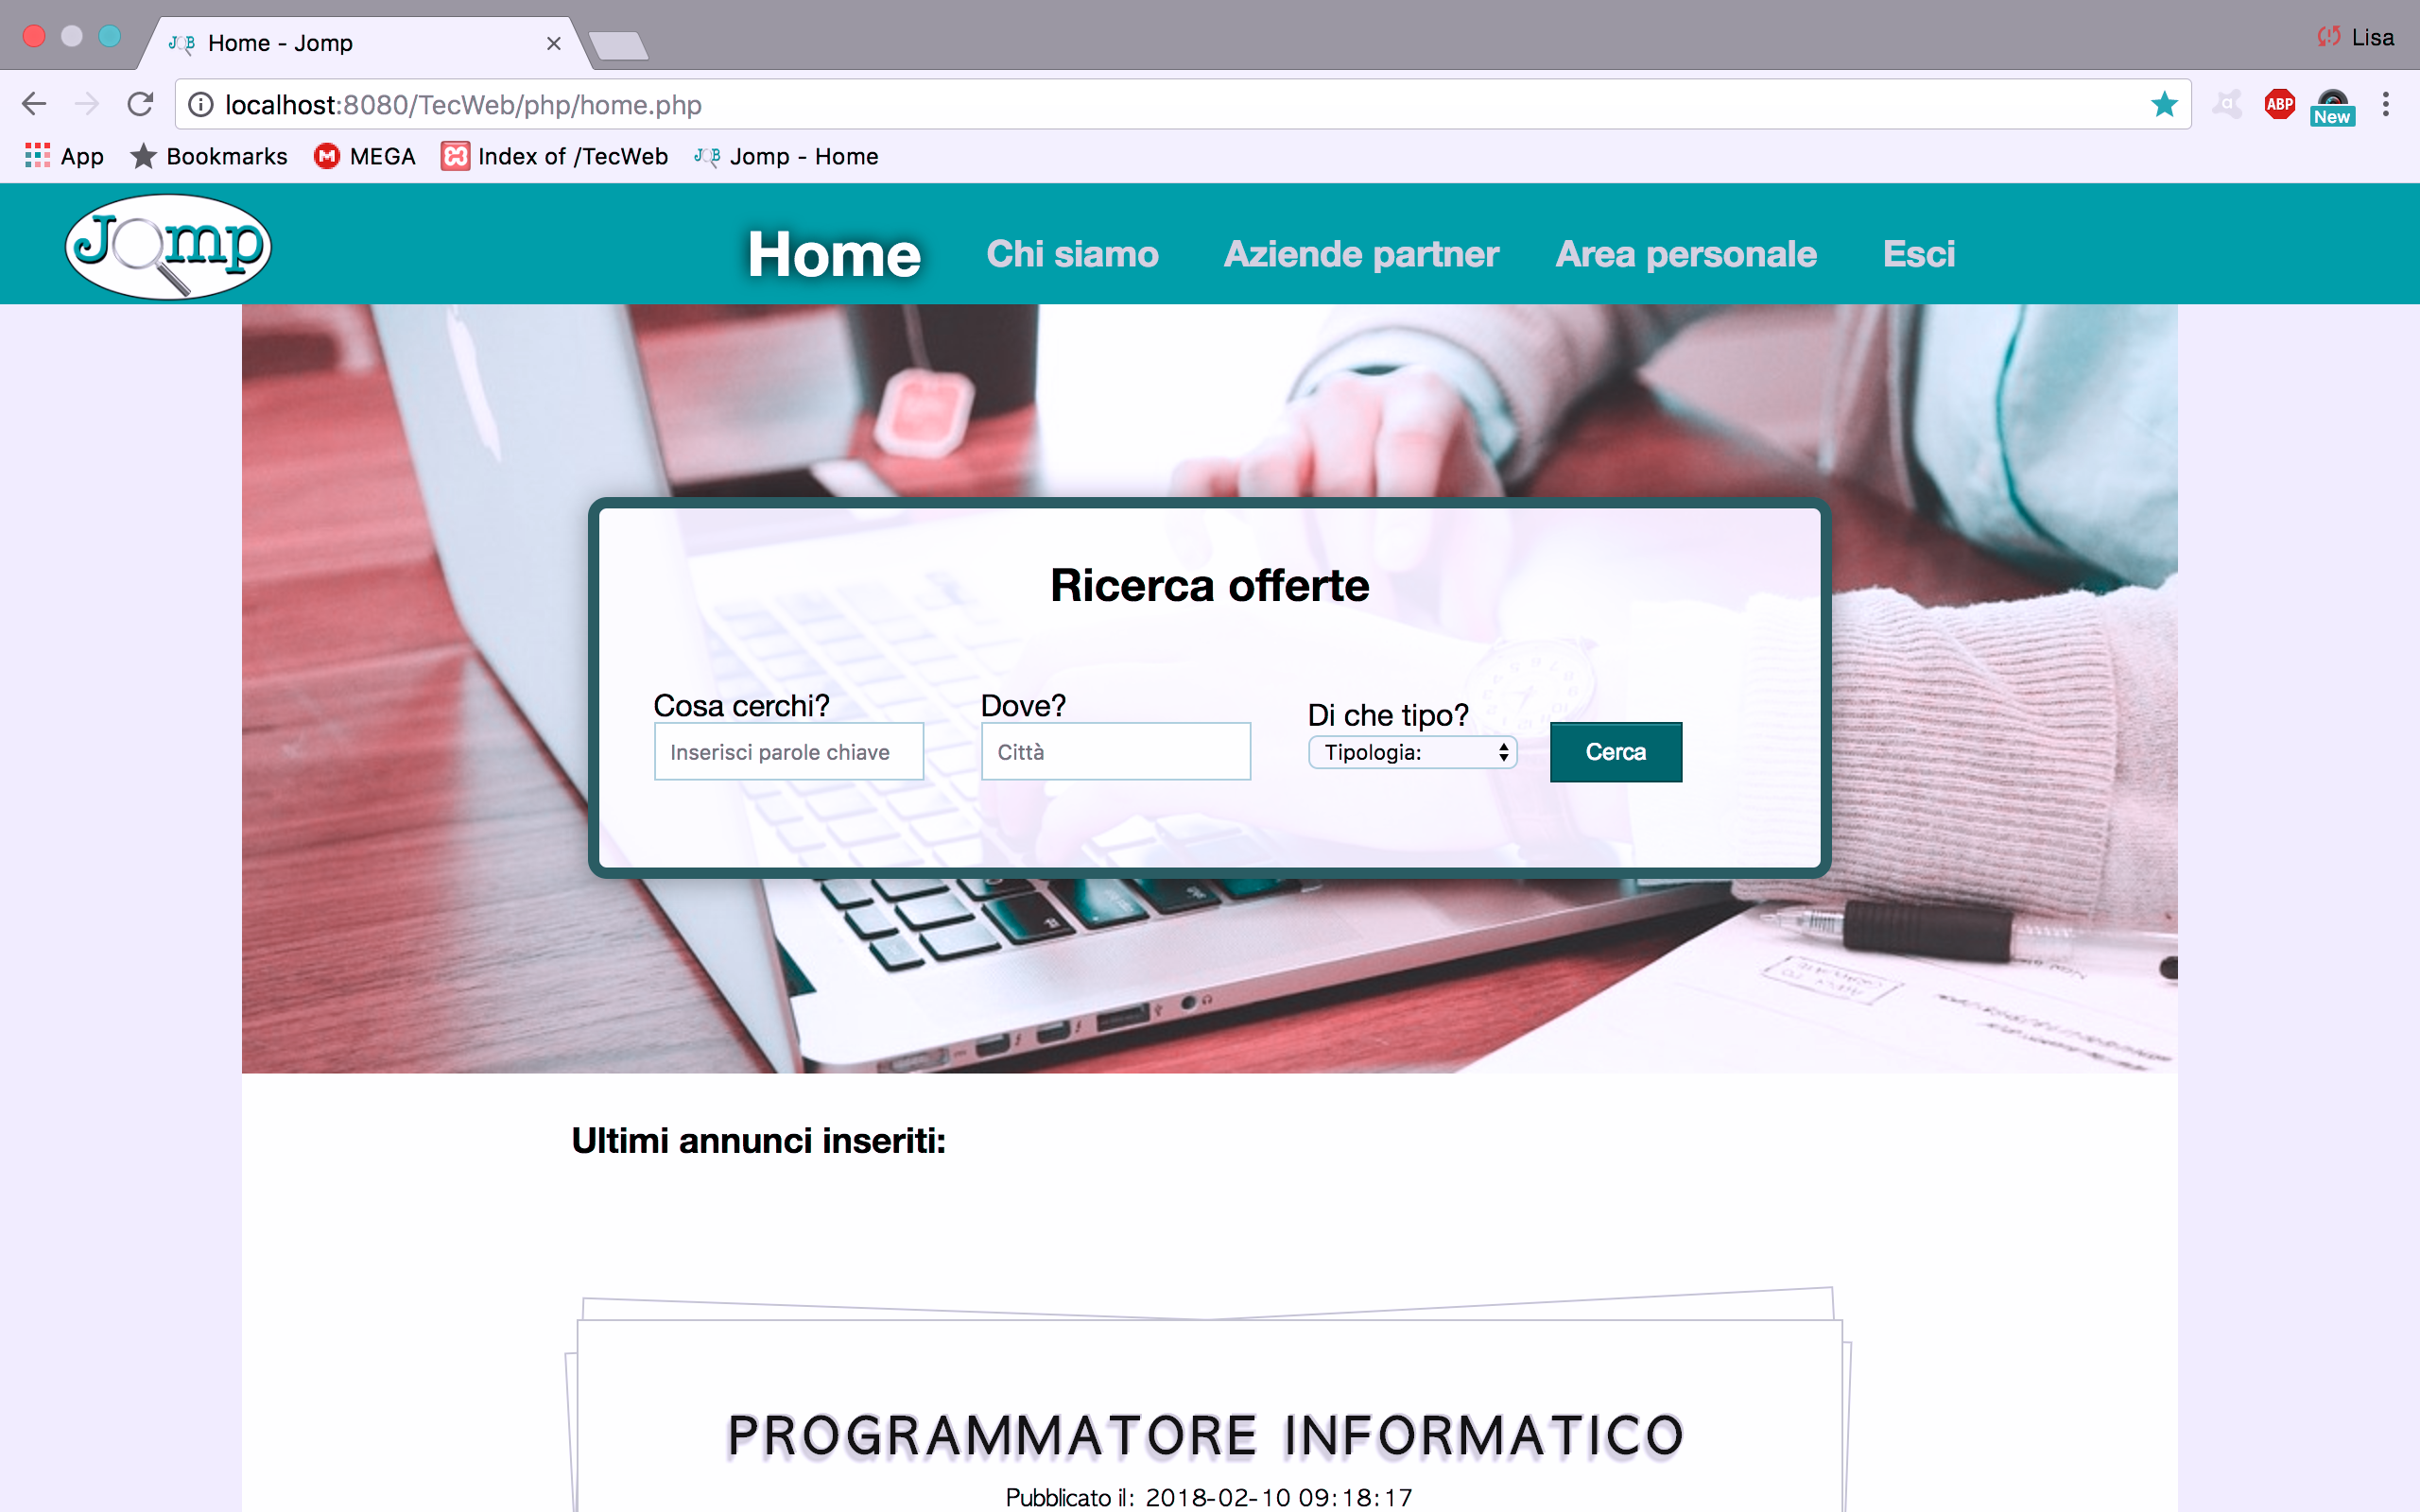
\includegraphics[scale=0.12]{Images/tritanopia.jpg}} 


	\subsection{Tag meta}
	Nell'head di ogni pagina sono stati inseriti  i tag \textit{meta}:  \textit{keywords}, \textit{description}, \textit{author} e \textit{languages} e il tag \textit{title}, il quale descrive la pagina corrente \textbf{dal particolare al generale}. Il tag \textit{languages} indica che il sito è stato interamente scritto in italiano ma compaiono alcune parole inglesi, le quali sono state affiancate dall’attributo: \textit{xml:lang=”en”}.
	
	\subsection{Screen reader}
	Ogni immagine presente nel sito è stata dotata degli attributi \textit{alt} e \textit{title} che descrivono in maniera esaustiva ciò che l'immagine ritrae. Per le immagini che sono state ritenute non di contenuto, e che sono così state inserite tramite CSS, non è stato previsto l'uso di questi attributi, poiché la loro unica funzione è di presentazione, non portando valore aggiunto al contenuto.
	Ogni campo di un form è stato sempre corredato con una etichetta \textit{label}.
	
	\subsection{Aiuti per la navigazione}
	Al fine di aumentare l'accessibilità del sito sono previsti le seguenti facilitazioni per la navigazione:
	\begin{itemize}
		\item \textbf{Colori dei link}: per evitare il disorientamento durante la navigazione, sono previsti colori differenti per i link attivi visitati (\textbf{blue}) e quelli non visitati (\textbf{viola});
		\item \textbf{Tabindex}: ad ogni pressione del tasto tab il focus si sposta sul link direttamente successivo per agevolare la navigazione. Sono stati ridefiniti gli attributi \textit{tabIndex} dei link in modo da rispecchiare l'ordine desiderato;
		\item \textbf{Menù fisso}: Per facilitare la navigazione nel sito è stato fissato il menù sopra la pagina così che l'utente possa sempre cambiare pagina senza dover tornare all'inizio di quella corrente per accedere al menù..
	\end{itemize}
	


